\documentclass{article}
\usepackage[margin=1in]{geometry}
\usepackage{mymathstyle}
\usepackage{algorithm2e}
\usepackage{graphicx}

\usepackage{tikz}
\usetikzlibrary{positioning}
\pgfmathtruncatemacro\distance{1}
\usepackage{fp}


\usepackage[style=authoryear,backend=biber,url=false,isbn=false]{biblatex}
\addbibresource{references.bib}

\title{Relational Convolution Networks}
\author{Awni \& John}
\date{Date created: June 27, 2023\\Last edited: \today}

\begin{document}
\maketitle

\section{Introduction}
\section{Introduction}\label{sec:intro}


%\begin{itemize}
%    \item The importance of relational learning; lots of references.
%    \item We propose a framework analogous to CNNs, but for relational learning
%    \item Advantages: modularity, compositionality, hierarchical.
%    \item Experiments showing advantages over existing frameworks. 
%    \item Main contribution: Framework for relational learning that shares the %strengths of CNNs for relational learning
%\end{itemize}

Modeling of relations between objects is important to a range of machine learning problems. For instance, an image analysis application might rely on comparing objects in terms of relations that extract color, size, or texture features; a natural language task may use relations that are based on syntactic or semantic features of pairs of words. While some machine learning tasks are ``purely relational'' and rely exclusively on identification and processing of relational information, others combine extraction of relations with function approximation.

To enable efficient learning of relational information, it is important to explore learning architectures that support processing of relations in a natural, expressive, and efficient manner. In this paper we propose a framework we call ``relational convolution networks.'' Our framework provides for relational representation learning what standard convolutional neural networks provide for typical image processing applications---a natural, expressive architecture for extracting hierarchical features of the raw data that can be used for building flexible prediction algorithms.

A schematic of the proposed architecture to support hierarchical relational learning is shown in Figure~\ref{fig:relconv_architecture}. Beginning with embeddings of objects, a multi-head relation module takes a sequence of embedded objects as input and produces a tensor that represents the relations between each pair of objects. The relational convolution layer then transforms the relation tensor into a sequence of new objects, each describing the relations within some group of objects at the previous layer.  An important component of the architecture is to use ``graphlets'' to carry out the relational convolution operation over groupings of the objects. Analogous to filters in CNNs, relational graphlets form a template of relations between subsets of objects against which the relation tensor is compared. The next layer receives this sequence of new objects as input and again models the relations within it. Thus, each layer computes relational features of a higher order---that is, relations on relations. This is analogous to the manner in which convolutional layers in a CNN can be composed to construct a chain of feature maps.

In a series of experiments, we show how relational convolutional neural networks provides an effective framework (and inductive bias) for relational learning. We first carry out experiments on ``relational games" proposed as a benchmark for relational reasoning by~\citep{shanahanExplicitlyRelationalNeural}. This consists of a suite of binary classification tasks for identifying abstract relational rules between a set of objects represented as images. We next carry out experiments on a version of the SET game, which requires processing of  higher-order relations between multiple attributes on a set of cards. For both tasks, relational convolutional networks are able to achieve more sample efficient learning compared to Transformers, as well as other architecture that have been specifically developed for relational learning.

\begin{wrapfigure}{R}{0.5\textwidth}
    \centering
    \includegraphics[width=.5\textwidth]{figs/relconv_architecture.pdf}
    \caption{Proposed architecture for relational convolutional networks. Hierarchical relations are modeled by iteratively computing pairwise relations between objects and convolving the resultant relation filter with graphlet filters representing templates of relations between subsets of objects.}
    % At each layer, the multi-head relation module takes a sequence of objects as input and produces a relation tensor representing the relations between each pair of objects. The relational convolution layer then transforms the relation tensor into a sequence of objects each describing the relations within some group of objects at the previous layer. The next layer receives this sequence of objects as input and again models the relations within it. Thus, each layer computes relational features of a higher order (i.e., relations on relations). \textit{Legend}: $d_l$ represents the dimension of the objects at layer $l$; $z_i^{(l)}$ is the $i$th object at the $l$th layer; $R^{(k)}$ is the relation tensor at layer $l$; $r_l$ is the dimension of the relations at layer $l$; $n_l$ is the number of objects at layer $l$. \awni{can we cut down on the caption a bit for space?} \awni{should I make the modules different colors?}}\label{fig:relconv_architecture}
\end{wrapfigure}

\subsection{Related Work}

Several previous works have considered the design of machine learning architectures which support the representation of relational information, in various forms~\citep{battagliaRelationalInductiveBiases2018,palmRecurrentRelationalNetworks2018,zhangRAVENDatasetRelational2019}.

\textbf{Graph Neural Networks.} Graph neural networks (GNNs) are a class of neural network architectures which operate on graphs and process ``relational'' data~\citep{niepertLearningConvolutionalNeural2016,kipfSemiSupervisedClassificationGraph2017,schlichtkrullModelingRelationalData2017,velickovicGraphAttentionNetworks2017,kipfNeuralRelationalInference2018}. A defining feature of the GNN model is its use of a form of neural message-passing, wherein the hidden representation of a node is updated as a function of the hidden representations of its neighbors~\citep{gilmerNeuralMessagePassing2017}. Typical examples of tasks which GNNs are applied to include node classification, graph classification, and link prediction~\citep{hamiltonGraphRepresentationLearning2020}. %This is a very general model which includes as a special case convolutional neural networks, where the graph is a grid, and Transformers, where the graph is a complete graph and the message-passing function is a convex sum of the neighbors' representations. In our experiments, we compare to Transformers as a representative of the GNN model.

In GNNs, the `relations' are given to the model via edges in a graph. In contrast, our architecture, as well as the explicitly relational architectures described below, operate on collections of objects without any relations given as input. Instead, such relational architectures must infer the relevant relations from the objects themselves. Still, graph neural networks can be applied to relational tasks by passing in the collection of objects along with a complete graph. A Transformer Encoder can be thought of as a special case of this architecture.%, and hence is the representative baseline we compare against in our experiments.

\textbf{Attention as modeling relations} Several works have proposed architectures with the ability to model relations by incorporating an attention mechanism~\citep{vaswani2017attention,locatelloObjectCentricLearningSlot2020,santoroRelationalRecurrent2018,zambaldiDeepReinforcementLearning2018,velickovicGraphAttentionNetworks2017}. Attention mechanisms model relations between objects implicitly as an intermediate step in a form of neural message-passing in order to update the representation of each object as a function of its context.

\textbf{Emerging literature on ``explicitly relational'' architectures.} There exists a growing literature on neural architectures which aim to explicitly model relational information between objects. An early example is~\citep{santoroSimpleNeural2017}.~\citet{shanahanExplicitlyRelationalNeural} proposes the PrediNet architecture, which aims to learn relational representations which are compatible with predicate logic.~\citet{webbEmergentSymbols2021} proposes ESBN, a recurrent neural network augmented with external memory with a memory-write operation which factors representations into `sensory' and `relational'.~\citet{kergNeuralArchitecture2022} proposes CoRelNet, a simple architecture based on `similarity scores' which aims to distill the relational inductive biases discovered in previous work into a minimal architecture.~\citet{altabaaAbstractorsTransformer2023} explored relational inductive biases in the context of Transformers, and proposed a view of relational inductive biases as a type of selective ``information bottleneck'' which disentangles relational information from object-level features.~\citet{webbRelationalBottleneckInductive2023} provides a cognitive science perspective on this idea, arguing that a relational information bottleneck may be a mechanism for abstraction in the human mind.% and brain.

We aim to contribute to this literature by proposing a framework for learning hierarchical relational representations through a natural compositional architecture. %in a natural, interpretable, sample-efficient, and parameter-efficient manner.

\section{Multi-Head Relational Layer: modeling relations via inner products}
\section{Multi-Head Relational Layer: modeling relations via inner products}\label{sec:mhr}

A relation function is a function which maps a pair of objects $o_1, o_2 \in \calX$ to a vector representing the relation between the two objects. For example, a relation may represent the information ``object 1 has the same color as object 2'', ``object 1 is larger than object 2'', and ``object 1 is to the left of object 2''. In principle, this can be modeled by an arbitrary learnable function on the concatenation of the two objects' representations. For example,~\citep{santoroSimpleNeural2017} models relations by MLPs applied to the concatenation of pairs of objects, $g_\theta(o_1, o_2)$. While this approach may work in some cases, it is missing some crucial inductive biases. In particular, there is no restriction that the learned pairwise function is in fact \textit{relational}. That is, $g_\theta(o_1, o_2)$ may just as well represent non-relational information like ``$o_1$ is bright'' and ``$o_2$ is small'', as opposed to relational information like ``$o_1$ is the same color as $o_2$'' and ``$o_1$ is larger than $o_2$''.

Recent work has explored using \textit{inner products} to model relations between objects~\citep{webbEmergentSymbols2021, kergNeuralArchitecture2022, altabaaAbstractorsTransformer2023}. The advantage of such an approach is that it provides added pressure to learn explicitly relational functions. In particular, it induces a geometry on the object space $\calX$ which allows objects to be described in relation to each other. To see this, we can first consider the case of symmetric relations modeled as inner products between feature maps. Let $\phi: \calX \to \reals^d$ be some feature map which represents a particular attribute of the object (e.g., color). Then, the inner product $\iprod{\phi(o_1)}{\phi(o_2)}$ induces a metric on $\calX$. In fact, $\iprod{\phi(o_1)}{\phi(o_2)}$ turns $\calX$ into an inner product space with well-defined notions of distance, angles, and orthogonality. Thus, we can say that the attribute $\phi$ is similar between two objects $o_1, o_2$ when the inner product $\iprod{\phi(o_1)}{\phi(o_2)}$ is large.

More generally, we can allow for multi-dimensional relations by having multiple encoding functions prior to the inner product. Furthermore, we can allow for asymmetric relations by having different encoding functions for the first and second object. This is the approach we take in~\citep{altabaaAbstractorsTransformer2023}. In particular, we model relations by,
\begin{equation}\label{eq:relation_function}
    r(x, y) = \begin{pmatrix}
        \iprod{\phi_1(x)}{\psi_1(y)} \\
        \vdots \\
        \iprod{\phi_{d_r}(x)}{\psi_{d_r}(y)}
    \end{pmatrix} \in \reals^{d_r},
\end{equation}

\noindent where $\phi_1, \psi_1, \ldots, \phi_{d_r}, \psi_{d_r}$ are learnable functions. For each dimension $k \in [d_r]$ of the relation function, the maps $\phi_k, \psi_k$ extract a particular attribute of the objects which is then compared by the inner product.

To promote weight sharing, we can have one common non-linear map $\phi$ across all dimensions along with different linear maps for each object and each dimension of the relation. That is, 

\begin{equation}\label{eq:relation_function_lin_proj}
    r(x, y) = \begin{pmatrix}
        \iprod{W_1^{(1)}\phi(x)}{W_2^{(1)}\phi(y)} \\
        \vdots \\
        \iprod{W_1^{(d_r)}\phi(x)}{W_2^{(d_r)}\phi(y)} \\
    \end{pmatrix},
\end{equation}

\noindent where the learnable parameters are $\phi$ and $W_1^{(k)}, \ldots, W_1^{(k)}, k \in [d_r]$. $\phi: \calX \to \reals^{d_\phi}$ may be an MLP, for example, and $W_1^{(k)}, W_2^{(k)}$ are $d_i \times d_\phi$ matrices. The class of functions realizable by~\Cref{eq:relation_function_lin_proj} is the same as~\Cref{eq:relation_function} but enables greater weight sharing.

The ``Multi-Head Relation'' module receives a sequence of objects $x_1, \ldots, x_m$ as input and models the pairwise relations between them by~\Cref{eq:relation_function_lin_proj}, returning an $m \times m \times d_r$ relation tensor describing the pairwise relations between each pair of objects. 

\section{Relational (Graphlet) Convolutions}
\newcommand{\softreliprod}[3]{\left\langle #1, #2 \, \vert \, #3 \right\rangle_\mathrm{rel}}
\newcommand{\reliprod}[2]{\left\langle #1, #2 \right\rangle_\mathrm{rel}}

\subsection{Relational convolutions with discrete groups}
Suppose that we have a sequence of objects $(x_1, ..., x_n) \in (\mathbb{R}^{d})^m$ and a relation tensor $R \in \mathbb{R}^{n \times n \times d_r}$ describing the pairwise relations between them. $R$ should be thought of as obtained by a multi-head relation layer. The operation we will define does two things: 1) extracts relations between larger groups of objects using pairwise relations 2) transforms the relation tensor back into a sequence of objects, allowing it be composed with another relational layer.

Fix some filter size $s < n$, where $s$ is a hyperparameter of this grouping module/layer. One `filter' is given by the `graphlet' $f_1 \in \mathbb{R}^{s \times s \times d_r}$. This is a template for a `relation tensor' between $s$ objects. Note that the dimension of the relations in this filter matches that of the input relation tensor (i.e., the same $d_r$). Let $g \subset [n]$ be a subset of the objects $1, \ldots, m$ of size $s$. Suppose for now that $g$ is an ordered set (i.e., the group $(1, 2, 3)$ is different from the group $(2, 3, 1)$). Then, denote the relation tensor given by this (ordered) subset by $R[g] := [R[i,j]]_{i,j \in g}$. We define the relational inner product between this relation subtensor and the filter $f_1$ by
\begin{equation}
    \label{eq:relational_inner_prod_one_filt}
    \reliprod{R[g]}{f_1} \coloneqq \sum_{i,j \in g} \iprod{R[i,j]}{f_1[i,j]}_{\reals^{d_r}} = \sum_{i,j \in g} \sum_{k \in [d_r]} R[i,j,k] f_1[i,j,k].
\end{equation}

This is simply the inner product in the corresponding euclidean space $\mathbb{R}^{s^2 d_r}$ when each tensor is flattened. We call $\iprod{\cdot}{\cdot}_{\mathrm{rel}}$ the `relational inner product'. This quantity represents how much the relations within the objects in $g$ match the relations in the template $f_1$.

% Another relevant configuration is when the relation tensor $R$ is assumed to be symmetric (i.e.: pairwise relations are symmetric). In this case, filters can be restricted to be symmetric, and can now be identified with the smaller space $\{f \in \mathbb{R}^{s \times s \times r}: f[i,j] = f[j,i] \ \forall i,j \}$. The definition of the relational inner product can be simplified in this case to $\langle R[g], f_1 \rangle_R \coloneqq \sum_{i \leq j \in g} \langle R[i,j], f_1[i,j] \rangle$.

The relational convolution layer has some number of filters, $n_f$, which is also a hyper-parameters. Denote the collection of filters by $\boldsymbol{f} = \paren{f_1, \ldots, f_{n_f}} \in \reals^{s \times s \times d_r \times n_f}$, which we call a \textit{relational graphlet filter} (`relational' because it describes relations, `graphlet' because it corresponds to a subset of the $m$ objects, and filter because it is a template against which the relation tensor is compared). We define the relational inner product of a relation subtensor $R[g]$ with a relational graphlet filter $\bm{f}$ as the $n_f$-dimensional vector consisting of the relational inner products with each filter,
\begin{equation}
    \label{eq:relational_inner_prod}
    \reliprod{R[g]}{\bm{f}} \coloneq \begin{pmatrix} \reliprod{R[g]}{f_1} \\ \vdots 
 \\ \reliprod{R[g]}{f_{n_f}} \end{pmatrix} \in \mathbb{R}^{n_f}
\end{equation}

This vector summarizes various aspects of the relations within a group, captured by several different filters. We have overloaded notation, but will use the convention that a collection of filters is denoted by a bold symbol to distinguish between the two forms of the relational inner product. Each filter corresponds to one dimension in the final relation-summarizing vector for the group $g$. This is reminiscent of convolutional neural networks, where each filter gives us one channel in the output tensor.

We can also define a symmetric variant of the relational inner product which is invariant to the ordering of the elements in $g$. This can be done by pooling over all permutations of $g$. In particular, we suggest max-pooling and average-pooling, although any set-aggregator would be valid. We denote the permutation-invariant relational inner product by $\iprod{R[g]}{f_1}_{\mathrm{rel}, \mathrm{sym}}$,
\begin{equation}\label{eq:symmetric_relational_inner_prod}
    \iprod{R[g]}{\bm{f}} \coloneq \mathrm{Pool}\paren{\set{\reliprod{R[g']}{\bm{f}} \colon g' \in g!}},
\end{equation}
\noindent where $g!$ denotes the set of permutations of the group $g$. Recall that each $\iprod{R[g']}{\bm{f}}_{\mathrm{rel}}$ is $n_f$ dimensional, and the pooling is done independently for each dimension.

For a given group $g \subset [m]$, the relational inner product with a graphlet filter, $\iprod{R[g]}{\bm{f}}_\mathrm{rel}$, gives us a vector summarizing the relational patterns inside that group. We aim to get a sequence of objects which each describes the relational pattern within a particular group. Let $\calG$ be a set of size-$s$ groups of the the $m$ objects. The relational convolution between a relation tensor $R$ and a relational graphlet filter $\bm{f}$ is the sequence of relational inner products with each group in $\calG$,

\begin{equation}
    \label{eq:relational_convolution}
    R \ast \bm{f} \coloneq \left( \reliprod{R[g]}{\boldsymbol{f}} \right)_{g \in \calG} \equiv \left(z_1, ..., z_{\abs{\calG}}\right) \in (\mathbb{R}^{n_f})^{\abs{\calG}}
\end{equation}

Depending on whether we want groupings to be order-invariant, we may let $\calG$ be either the set of all permutations of size $s$ or the set of all combinations of size $s$ and use the corresponding definition of the relational inner product (i.e.,~\Cref{eq:relational_inner_prod} or~\Cref{eq:symmetric_relational_inner_prod}).

One important advantage of the relational convolution operation is its interpretability. The filters $\bm{f} = (f_1, \ldots, f_{n_f})$ are each a particular pattern of relations between $s$ objects. Furthermore, each object in the relational convolution $R \ast \bm{f}$ represents the degree to which the relations in the group $g$ match the patterns in each filter.

In the above, we either consider all possible groups or we somehow assume that the relevant groups $\calG$ are known and given. We may also wish to \textit{learn} the relevant groups.

\begin{figure}[!ht]
    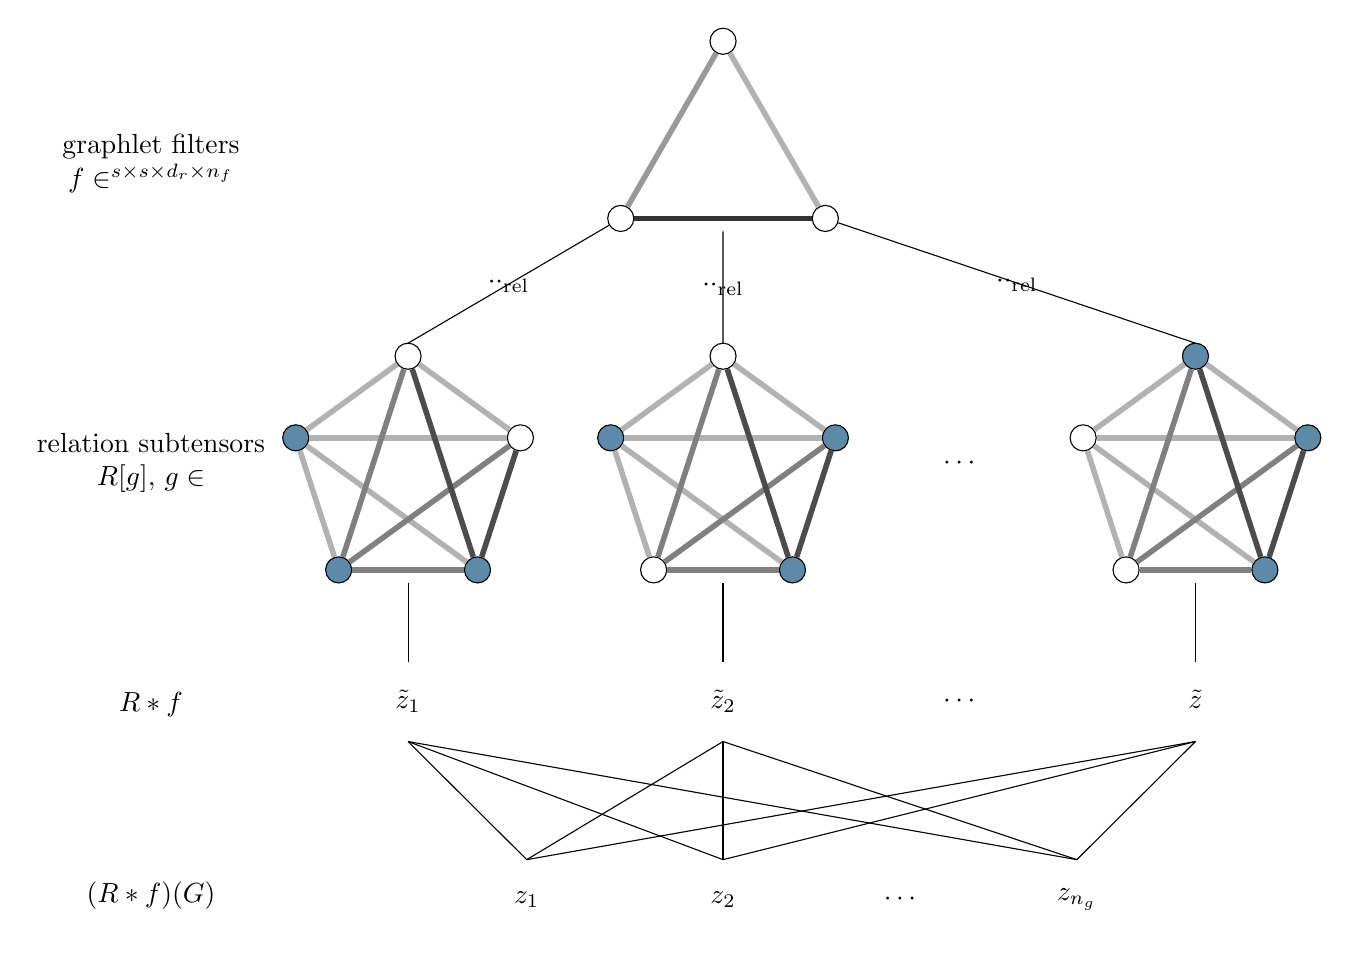
\begin{tikzpicture}[node distance=2cm]


% parameters
\definecolor{highlightcolor}{rgb}{0.36, 0.54, 0.66}
\def\edgethickness{2}
\def\edgeOpacity{{30, 50, 70, 30, 50}}
\def\nodeColors{{"highlightcolor", "highlightcolor", "highlightcolor", "white", "white"}}
\def\graphsize{1.5}

% first graph
\begin{scope}[local bounding box=graph1]
    % Nodes
    \foreach \i in {1,...,5} {
        \pgfmathsetmacro\color{\nodeColors[\i-1]};
        \node[circle, draw, fill=\color] (N1\i) at (90+\i*72:\graphsize) {};
    }

    % Edges
    \foreach \i in {1,...,5} {
        \foreach \j in {1,...,5} {
            \ifnum\i<\j
                \pgfmathtruncatemacro\index{\i-1}
                \pgfmathsetmacro\opacity{\edgeOpacity[\index]}
                \draw[black!\opacity, line width=\edgethickness pt] (N1\i) -- (N1\j);
            \fi
        }
    }
\end{scope}

% second graph
\def\nodeColors{{"highlightcolor", "white", "highlightcolor", "highlightcolor", "white"}}
\begin{scope}[shift={(4,0)}, local bounding box=graph2]
    \foreach \i in {1,...,5} {
        \pgfmathsetmacro\color{\nodeColors[\i-1]};
        \node[circle, draw, fill=\color] (N2\i) at (90+\i*72:\graphsize) {};
    }
    % Edges
    \foreach \i in {1,...,5} {
        \foreach \j in {1,...,5} {
            \ifnum\i<\j
                \pgfmathtruncatemacro\index{\i-1}
                \pgfmathsetmacro\opacity{\edgeOpacity[\index]}
                \draw[black!\opacity, line width=\edgethickness pt] (N2\i) -- (N2\j);
            \fi
        }
    }
\end{scope}

% third graph
\def\nodeColors{{"white", "white", "highlightcolor", "highlightcolor", "highlightcolor"}}
\begin{scope}[shift={(10,0)}, local bounding box=graph3]
    \foreach \i in {1,...,5} {
        \pgfmathsetmacro\color{\nodeColors[\i-1]};
        \node[circle, draw, fill=\color] (N3\i) at (90+\i*72:\graphsize) {};
    }
    % Edges
    \foreach \i in {1,...,5} {
        \foreach \j in {1,...,5} {
            \ifnum\i<\j
                \pgfmathtruncatemacro\index{\i-1}
                \pgfmathsetmacro\opacity{\edgeOpacity[\index]}
                \draw[black!\opacity, line width=\edgethickness pt] (N3\i) -- (N3\j);
            \fi
        }
    }
\end{scope}

% graphlet filter
\def\triangleSize{1.5} % Set the desired size of the triangle
\begin{scope}[shift={(4,4)}, local bounding box=triangle]
    % nodes
    \foreach \i in {1,...,3} {
        \node[circle, draw] (T\i) at (90+\i*120:\triangleSize) {};
    }
    % edges
    \draw[black!80, line width=\edgethickness pt] (T1) -- (T2);
    \draw[black!40, line width=\edgethickness pt] (T1) -- (T3);
    \draw[black!30, line width=\edgethickness pt] (T2) -- (T3);
\end{scope}

\draw (T1) -- (graph1.north) node[midway] {$\iprod{\cdot}{\cdot}_\mathrm{rel}$};
\draw (triangle.south) -- (graph2.north) node[midway] {$\iprod{\cdot}{\cdot}_\mathrm{rel}$};
\draw (T2) -- (graph3.north) node[midway] {$\iprod{\cdot}{\cdot}_\mathrm{rel}$};
\path (graph2.east) -- (graph3.west) node[midway] {$\cdots$};

\node [minimum size=1cm, below=1cm of graph1.south] (tz1) {$\tilde{z}_1$};
\node [minimum size=1cm, below=1cm of graph2.south] (tz2) {$\tilde{z}_2$};
\node [minimum size=1cm, below=1cm of graph3.south] (tzng) {$\tilde{z}_{\abs{\calG}}$};

\draw (graph1.south) -- (tz1.north);
\draw (graph2.south) -- (tz2.north);
\draw (graph3.south) -- (tzng.north);

\node [minimum size=1cm, below right=1.5cm and 1cm of tz1.south] (z1) {$z_1$};
\node [minimum size=1cm, below=1.5cm of tz2.south] (z2) {$z_2$};
\node [minimum size=1cm, below left=1.5cm and 1cm of tzng.south] (zng) {$z_{n_g}$};
\path (tz2.east) -- (tzng.west) node[midway] {$\cdots$};

\draw (tz1.south) -- (z1.north);
\draw (tz1.south) -- (z2.north);
\draw (tz1.south) -- (zng.north);
\draw (tz2.south) -- (z1.north);
\draw (tz2.south) -- (z2.north);
\draw (tz2.south) -- (zng.north);
\draw (tzng.south) -- (z1.north);
\draw (tzng.south) -- (z2.north);
\draw (tzng.south) -- (zng.north);
\path (z2.east) -- (zng.west) node[midway] {$\cdots$};

\node [left=0.1cm of graph1.west, align=center] (relsubtensors) {relation subtensors\\ $R[g],\, g \in \calG$};
\node [left=of tz1, below=6.5em of relsubtensors] (relconv) {$R \ast \bm{f}$};
\node [left=of z1, below=5.25em of relconv] (relconvsoft) {$(R \ast \bm{f})(G)$};
\node [left=of triangle, above=8em of relsubtensors,  align=center] (filters) {graphlet filters \\ $\bm{f} \in \reals^{s \times s \times d_r \times n_f}$};

\end{tikzpicture}
    \caption{A depiction of the graphlet relational convolution operation. The input is a relation tensor $R$ of shape $m \times m \times d_r$, giving pairwise relations of dimension $d_r$ between a sequence of $m$ objects. A graphlet filter of size $s$ is parameterized by a relation tensor of shape $s \times s \times d_r$. The graphlet convolution operation computes relational inner products for each of $n_f$ graphlet filters, $\bm{f}$. This gives a vector representation, $z_i \in \reals^{n_f}$, for each discrete group of $s$ objects. Finally, this is synthesized into a vector representation for each of $n_g$ `soft groups', $G$. The overall operation is denoted by $(z_1, \ldots, z_{n_g}) = (R \ast \bm{f})(G)$.}\label{fig:relconvdiagram}
\end{figure}


\subsection{Relational convolutions with `soft' groups}

In the above formulation, the groups are `discrete', and we consider every possible group. Having discrete groups can be nice for interpretability. But, one challenge we face here is that the number of objects grows rapidly after applying this module. That is, the number of groups to consider $\abs{\calG} = \binom{m}{s}$ may be intractably large, especially if the number of input objects $n$ is large. This may pose computational issues. Furthermore, considering every possible grouping may be unnecessary and may make learning more difficult.

In order to address these issues, we might want to explicitly model the groups. This allows us to control the number of objects in the output sequence such that only useful groups are considered.

In the next section, we outline some ways to model `soft groups' using \textit{Grouping Layers}. These layers take a sequence of objects and/or the relation tensor as input and produce a group matrix $G \in \reals^{m \times n_g}$ representing $n_g$ `soft groups'. The $(i,j)$th entry of the group matrix represents the degree to which the $i$th object belongs to the $j$th group. The number of groups $n_g$ is a configurable hyperparameter of the grouping layers. The groups may be a function of the position of the objects in the sequence, the features of the objects, and/or the relations between objects. Different grouping schemes may be more or less appropriate for different tasks. This is discussed in detail in the next section. For now, we assume that the group matrix $G$ is given as input the relational convolution layer.

Consider the group matrix $G \in \reals^{m \times n_g}$ and filters $\bm{f}$ of size $s$. First, we use $G$ to compute a ``group-match score'' for each discrete group $g$ of size $s$ (e.g., $g \in \calG = \binom{[m]}{s}$). This is done via

\begin{equation}
    \label{eq:group_match_score}
    \begin{split}
        G &\gets \text{SoftPlus}(G)\\
        \alpha_{gk} &\gets \text{Softmax}\paren{\paren{\prod_{i \in g} G[i,k]}_{g \in \calG}}, \quad g \in \calG, k \in [n_g],
    \end{split}
\end{equation}

where the soft-plus function is $\text{Softplus}(x) = \log(\exp(x + 1))$, applied elementwise. This has the effect of making the group matrix $G$ non-negative which is needed for the product of its elements to represent a ``group-match score''. The product inside the softmax is over elements in the discrete group $g \in \calG$. Hence, it will be large whenever the softgroup $G[:, k]$ aligns with the discrete group $g$. Thus, $\alpha_{gk}$ is a normalized ``group-match score'' indicating the degree to which the discrete group $g$ matches the given soft group $G[:,k]$. Note that the group match scores of discrete groups sum to one: $\sum_{g \in G} \alpha_{gk} = 1, \ \forall k \in [n_g]$.

Now, we can define the `soft' relational inner product given the `soft' group $G_k = G[:, k]$ by
\begin{equation}
    \label{eq:soft_relational_inner_prod}
    \langle R, \boldsymbol{f} \, \vert \, G_k \rangle_R \coloneqq \sum_{g \in \calG} \alpha_{gk} \iprod{R[g]}{\boldsymbol{f}}_\mathrm{rel}
\end{equation}

This notation should be read as ``the relational inner product of the relation tensor $R$ with the graphlet filters $\boldsymbol{f}$ given the group $G_k$''. This expression is essentially a convex combination of the relational inner product with all possible discrete groups weighted by how much they match the soft group $G_k$.

With this modification, the number of objects in the output sequence is fixed and controlled by the number of groups, $n_g$ (which is a hyperparameter). The output sequence of the relational convolution given groups $G$ is now given by

\begin{equation}
    \label{eq:soft_relational_convolution_groups}
    (R \ast \bm{f})(G) = \left( \softreliprod{R}{\bm{f}}{G_1}, \ldots, \softreliprod{R}{\bm{f}}{G_{n_g}} \right) \in \left(\mathbb{R}^{n_f}\right)^{n_g}
\end{equation}

\comment{TODO: is this notation good?}

\subsection{Efficiency of `convolutions'}
The operation we have defined here is a `convolution' in the sense that we take a patch of the relation tensor, given by a group, and compare the relations within it to a template graphlet filter via an appropriately-defined inner product. This is similar to how, in a convolutional neural network, we would take a patch of an image and compare it to an image filter. Another similarity to CNNs is that the same graphlet filters are used for all groupings, thus enabling weight-sharing. This is similar to how the same convolutional filters are used for all image patches in a CNN. This makes our framework quite efficient when it comes to the number of parameters and, hopefully, makes learning easier.

% This connection extends to (message-passing) graph neural networks. A key difference however is the following. In a graph neural network, we compute a convolution \textit{along} the graph (i.e.: the graph is what determines a node's neighbors for message-passing). What we are proposing here is that we `convolve' the (relational) graph itself with another graph. 

This analogy motivates one possible style of architectures in our framework~\Cref{fig:relational_framework}. Namely, to have the number of groups after each relational-grouping module decrease while increasing the number of filters. This can be done until we obtain a single group with a long feature vector. This should give a representation of the relational features across all objects, including higher-order relational features (i.e., relations on relations). This single vector can then be passed to a dense feedforward network. This is similar to the ``fully convolutional network'' architecture, where the height and width of the tensor are iteratively decreased (by pooling layers) while increasing the number filters, resulting in a long and thin vector.



\section{Experiments}
\section{Experiments}\label{sec:experiments}

The \textit{relational games} dataset was contributed as a benchmark for relational reasoning by~\citep{shanahanExplicitlyRelationalNeural}. It consists of a family of binary classification tasks for identifying abstract relational rules between a set of objects represented as images. The objects consist of three sets of simple geometric shapes, referred to as ``pentominoes'', ``hexominoes'', and ``stripes'' (\Cref{fig:relational_games_objects}). The objects are arranged in a $3 \times 3$ grid. Each relational game task corresponds to some relationship between the objects (see~\Cref{tab:relational_games_tasks} and~\Cref{fig:relational_games_tasks}), and the target is to classify whether the relationship holds among a given sequence of objects or not.

In our experiments, we evaluate out-of-distribution generalization by training all models on the pentominoes objects and evaluating on the hexominoes and stripes objects. The input to all models is presented as a sequence of $9$ objects, each represented as a $12 \times 12 \times 3$ RGB image. In all models, the objects are processed independently by a CNN with a shared architecture. This produces a sequence of $9$ $d$-dimensional vectors. The sequence of objects is then passed to the relation-processing component of the model. The results are then flattened and passed through an MLP with a shared architecture to produce the final prediction. We compare four models: a relational convolution model (abbreviated RelConvNet), CoRelNet~\citep{kergNeuralArchitecture2022}, PrediNet~\citep{shanahanExplicitlyRelationalNeural}, and a Transformer~\citep{vaswani2017attention}. The architectural details of each model are described in~\Cref{tab:architectures}.

The pentominoes split of the relational games dataset is used for training. We hold out 1000 samples for validation (during training) and 5000 samples for testing (after training), and use the rest as the training set. The hexominoes and stripes splits are used to test out-of-distribution generalization after training. For each task and model, we train the model for 50 epochs, while tracking training and validation loss and accuracy. We use the categorical cross-entropy loss and the Adam optimizer with learning rate $0.001$, $\beta_1 = 0.9, \beta_2 = 0.999, \epsilon = 10^{-7}$. We use a batch size of 512. For each model and task, we run 5 trials with different random seeds.

\begin{table}[ht]
    \centering
    \begin{tabular}{p{0.2\textwidth}p{0.7\textwidth}}
    \toprule
    Task              & Description                                                                                                                                                                                             \\ \midrule
    \texttt{same}              & Two random cells out of nine are occupied by an object. They are the ``same'' if they have the same color, shape, and orientation (i.e., identical image)                                               \\\hline
    \texttt{occurs}            & The top row contains one object and the bottom row contains three objects. The ``occurs'' relationship holds if at least one of the objects in the bottom row is the same as the object in the top row. \\\hline
    \texttt{xoccurs}           & Same as occurs, but the relationship holds if exactly one of the objects in the bottom row is the same as the object in the top row.                                                                    \\\hline
    \texttt{between}           & The grid is occupied by three objects in a line (horizontal or vertical). The ``between'' relationship holds if the outer objects are the same.                                                         \\\hline
    \texttt{row match pattern} & The first and third rows of the grid are occupied by three objects each. The ``match pattern'' relationship holds if the relation pattern in each row is the same (e.g., AAA, AAB, ABC, etc.)           \\ \bottomrule
\end{tabular}

    \caption{Relational games tasks.}
    \label{tab:relational_games_tasks}
\end{table}

\begin{figure}
    \centering
    \begin{subfigure}[t]{0.37\textwidth}
        \centering
        \includegraphics[width=\textwidth]{figs/relational_games_objects.pdf}
        % \caption{Examples of objects from each split.}
        \label{fig:relational_games_objects}
    \end{subfigure}
    \begin{subfigure}[t]{0.62\textwidth}
        \centering
        \includegraphics[width=\textwidth]{figs/relational_games_tasks.pdf}
        % \caption{Examples of problem instances for each task. The top row is an example where the relation holds and the bottom row is an example where the relation does not hold.}
        \label{fig:relational_games_tasks}
    \end{subfigure}
    \caption{Relational games dataset.~\textbf{Left} Examples of objects from each split.~\textbf{Right} Examples of problem instances for each task. The top row is an example where the relation holds and the bottom row is an example where the relation does not hold.}
    \label{fig:relational_games_dataset}
\end{figure}

\begin{table}[ht]
    \centering
    \input{figs/experiments/architectures_table.tex}
    \caption{Model architectures.}
    \label{tab:architectures}
\end{table}



\begin{figure}
    \centering
    \includegraphics[width=\textwidth]{figs/experiments/all_training_curves.pdf}
    \caption{Training curves for each relational games task. Showing curves up to 2,000 batch steps. Solid lines indicate the mean over 5 trials and the shaded regions indicate a bootstrap 95\% confidence interval.}\label{fig:training_curves}
\end{figure}

\textbf{Sample efficiency.} We observe that the relational inductive biases of RelConvNet, and relational models more generally, grant a significant advantage in sample-efficiency.~\Cref{fig:training_curves} shows the training accuracy over the first 2,000 batches for each model. RelConvNet, CoRelNet, and PrediNet are explicitly relational architectures, whereas the Transformer is not. The Transformer is able to process relational information through its attention mechanism, but this information is entangled with the features of individual objects (which, for these relational tasks, is extraneous information). The Transformer consistently requires the largest amount of data to learn the relational games tasks. PrediNet tends to be more sample-efficient. RelConvNet and CoRelNet are the most sample-efficient, with RelConvNet only slightly more sample-efficient on the `same', `occurs', `xoccurs', and `between' tasks.

On the `match pattern' task, however, RelConvNet is significantly more sample-efficient. We attribute this to the fact that RelConvNet is able to model higher-order relations through its relational convolution module. The `match pattern' task can be thought of as a simple second-order relational tasks---it involves computing relations between two groups objects, and comparing those relations between the two groups. The relational convolution module naturally models this kind of situation since it considers groups of objects and describes the relations between them. The performance we observe here indicates that the relational games dataset is in some sense saturated by models like RelConvNet and CoRelnet and that more complex relational benchmarks are needed to evaluate this class of models. In particular, benchmarks which test the ability to model higher-order relations.

\begin{table}
    \centering
    \begin{tabular}{llll}
\toprule
              &                           &     Hexos Accuracy &   Stripes Accuracy \\
Task & Model &                    &                    \\
\midrule
same & CoRelNet &  $0.988 \pm 0.006$ &  $0.724 \pm 0.112$ \\
              & PrediNet &  $0.990 \pm 0.004$ &  $0.983 \pm 0.007$ \\
              & Transformer &  $0.997 \pm 0.001$ &  $0.993 \pm 0.004$ \\
              & RelConvNet &  $0.989 \pm 0.002$ &  $0.974 \pm 0.003$ \\
              & RelConvNet (Temporal G) &  $0.981 \pm 0.002$ &  $0.965 \pm 0.007$ \\
              & RelConvNet (Feature G) &  $0.985 \pm 0.001$ &  $0.978 \pm 0.006$ \\
              & RelConvNet (Contextual G) &  $0.981 \pm 0.002$ &  $0.969 \pm 0.012$ \\\hline
occurs & CoRelNet &  $0.992 \pm 0.004$ &  $0.518 \pm 0.012$ \\
              & PrediNet &  $0.907 \pm 0.020$ &  $0.775 \pm 0.046$ \\
              & Transformer &  $0.881 \pm 0.015$ &  $0.724 \pm 0.021$ \\
              & RelConvNet &  $0.980 \pm 0.001$ &  $0.880 \pm 0.015$ \\
              & RelConvNet (Temporal G) &  $0.983 \pm 0.001$ &  $0.920 \pm 0.012$ \\
              & RelConvNet (Feature G) &  $0.788 \pm 0.112$ &  $0.747 \pm 0.099$ \\
              & RelConvNet (Contextual G) &  $0.951 \pm 0.004$ &  $0.830 \pm 0.044$ \\\hline
xoccurs & CoRelNet &  $0.980 \pm 0.007$ &  $0.606 \pm 0.035$ \\
              & PrediNet &  $0.872 \pm 0.036$ &  $0.810 \pm 0.028$ \\
              & Transformer &  $0.867 \pm 0.017$ &  $0.753 \pm 0.031$ \\
              & RelConvNet &  $0.967 \pm 0.001$ &  $0.946 \pm 0.006$ \\
              & RelConvNet (Temporal G) &  $0.963 \pm 0.006$ &  $0.939 \pm 0.012$ \\
              & RelConvNet (Feature G) &  $0.760 \pm 0.107$ &  $0.754 \pm 0.103$ \\
              & RelConvNet (Contextual G) &  $0.942 \pm 0.020$ &  $0.901 \pm 0.029$ \\\hline
between & CoRelNet &  $0.995 \pm 0.001$ &  $0.582 \pm 0.063$ \\
              & PrediNet &  $0.978 \pm 0.006$ &  $0.950 \pm 0.019$ \\
              & Transformer &  $0.986 \pm 0.003$ &  $0.961 \pm 0.010$ \\
              & RelConvNet &  $0.991 \pm 0.001$ &  $0.988 \pm 0.002$ \\
              & RelConvNet (Temporal G) &  $0.992 \pm 0.001$ &  $0.979 \pm 0.004$ \\
              & RelConvNet (Feature G) &  $0.993 \pm 0.001$ &  $0.981 \pm 0.003$ \\
              & RelConvNet (Contextual G) &  $0.992 \pm 0.002$ &  $0.972 \pm 0.012$ \\\hline
match pattern & CoRelNet &  $0.942 \pm 0.011$ &  $0.581 \pm 0.026$ \\
              & PrediNet &  $0.710 \pm 0.040$ &  $0.658 \pm 0.053$ \\
              & Transformer &  $0.627 \pm 0.005$ &  $0.591 \pm 0.006$ \\
              & RelConvNet &  $0.961 \pm 0.015$ &  $0.870 \pm 0.041$ \\
              & RelConvNet (Temporal G) &  $0.979 \pm 0.003$ &  $0.967 \pm 0.002$ \\
              & RelConvNet (Feature G) &  $0.976 \pm 0.003$ &  $0.958 \pm 0.009$ \\
              & RelConvNet (Contextual G) &  $0.935 \pm 0.047$ &  $0.896 \pm 0.060$ \\
\bottomrule
\end{tabular}

    \caption{Out-of-distribution Generalization results on relational games. We report means $\pm$ standard error of mean over 5 trials.}\label{tab:ood_generalization}

\end{table}

\begin{figure}
    \begin{subfigure}{0.5\textwidth}
        \centering
        \includegraphics[width=\textwidth]{figs/experiments/hexos_acc.pdf}
        \caption{OoD generalization on Hexos objects}\label{fig:ood_generalization_hexos}
    \end{subfigure}
    \begin{subfigure}{0.5\textwidth}
        \centering
        \includegraphics[width=\textwidth]{figs/experiments/stripes_acc.pdf}
        \caption{OoD generalization on Stripes objects}\label{fig:ood_generalization_stripes}
    \end{subfigure}
    \caption{Out-of-distribution generalization on hold-out object sets. Bar heights indicate the mean over 5 trials and the errror bars indicate a bootstrap 95\% confidence interval.}\label{fig:ood_generalization}
\end{figure}

\textbf{Out-of-distribution generalization}~\Cref{fig:ood_generalization} and~\Cref{tab:ood_generalization} report model performance on the two hold-out object sets after training. On the hexominoes objects, which are similar-looking to the pentominoes objects used for training, RelConvNet and CoRelNet do nearly perfectly. PrediNet and the Transformer do well on the simpler tasks, but struggle with the more difficult `match pattern' task. The stripes objects are visually more distinct from the pentominoes of the training split, making generalization more difficult. We observe an overall drop in performance for all models. The drop is particularly dramatic for CoRelNet\footnote{Unlike~\citep{kergNeuralArchitecture2022}, we do not use temporal context normalization in our experiments. We believe this is the more appropriate choice for evaluating relational architectures such as RelConvNet and CoRelNet since TCN is an added confounder. We discuss this more in~\Cref{sec:tcn_discussion}.}. We conjecture that this is due to CoRelNet's inability to model multi-dimensional relations, necessitating that all relational information is squeezed into a scalar quantity. \texttt{TODO: elaborate or remove this comment?}. The separation between RelConvNet and the other models is largest on the ``match pattern'' task of the stripes split (the most difficult task and the most difficult generalization split). Here, RelConvNet maintain a mean accuracy of 87\% while the other models drop below 65\%. We conjecture that this is due to RelConvNet's natural ability to model such higher-order relations as well as its ability to model multi-dimensional relations.

\section{Grouping Layers}
\section{Grouping Layers}\label{sec:grouping_layers}

\textcolor{red}{remove this section if we use the alternate `soft groups' model.}

A grouping layer is a layer which outputs a group matrix $G \in \reals^{m \times n_g}$ representing the degree to which each object $i \in [m]$ belongs to each group $j \in [n_g]$. The number of groups $n_g$ is a configurable hyperparameter. We briefly describe some proposals for grouping layers with different properties.

\textbf{Temporal (Positional) Grouping.} In the temporal grouping layer, the groups are a function only of the temporal order of the objects. This can be achieved by learning the group matrix $G$ directly as a parameter of the model. $G$ will be optimized along with the rest of the model parameters as a function of its effect on the relational convolution layer. Temporal grouping would be appropriate in situations where the order in which objects appear is predetermined and indicates the relevant groups. For example, objects that are positionally close to each other may be grouped together.

\textbf{Feature-based Grouping.} In a feature-based grouping layer, the group(s) to which each object belongs is a function of that object's features (and position). That is,
\begin{equation}\label{eq:feat_grouping}
        G \gets \begin{bmatrix}
            \phi(1, x_1)^\top \\
            \vdots \\
            \phi(m, x_m)^\top
        \end{bmatrix} \in \reals^{m \times n_g},
\end{equation}

\noindent where $\phi: [m] \times \calX \to \reals^{n_g}$ is a learnable function which maps an object's temporal order $i$ and feature representation $x_i$ to a $n_g$-dimensional group membership vector where the $j$th entry of the vector represents the degree to which the object belongs to the $j$th group. For example $\phi$ can be a multi-layer perceptron of the form $\phi(i, x) = \mathrm{MLP}(\mathrm{concat}(e_i, x))$. Feature-based grouping may be useful in situations where group membership can be determined for each object using only that object's features, irrespective of the context of the other objects in the sequence.

\textbf{Context-aware Grouping.} In some applications, the group(s) to which each object belongs to may depend on the full context of the other objects in the sequence. One way to model this is to use a message-passing neural network to update the representations of each object, incorporating the context of the other objects in the sequence. Then, a multi-layer perceptron is applied to each encoded object to produce the group membership vector for that object.
\begin{equation}\label{eq:context_grouping}
    \begin{split}
        E_i &\gets \mathrm{MessagePassing}\paren{x_i, \set{x_1, \ldots, x_m}}, \ i \in [m] \\
        G &\gets \begin{bmatrix}\mathrm{MLP}(E_1)^\top \\ \vdots \\ \mathrm{MLP}(E_m)^\top \end{bmatrix} \in \reals^{m \times n_g}.
    \end{split}
\end{equation}

This is the most general form of grouping, as it encompasses the previous two forms as special cases. The updated representation of each object $E_i$ now contains any relevant information about the other objects which should be considered in computing its group membership vector. One simple and effective option for the message-passing operation is to use self-attention. In this case, since an inner product relation layer precedes the relational convolution layer, the relation tensor can be re-used in the self-attention operation to compute attention scores.

\section{Function Class of Multi-Head Relation Module}
In previous work, we characterized the class of functions which can be modeled by \textit{symmetric} multi-head relation modules~\parencite{altabaaAbstractorsTransformer2023}. In particular, we showed that this class of functions is the set of relation functions which are symmetric kernels of positive type (i.e., Mercer kernels) in each relation dimension.

Symmetric relation functions modeled in this way are natural \textit{measures of similarity}. To see this, suppose we have a normalized symmetric positive definite kernel $K$, such that $K(x,x) = 1$ for all $x \in \calX$. Then, the Cauchy-Schwarz inequality for Mercer kernels states that
\begin{equation}
    K(x, y)^2 \leq K(x, x) K(y, y) = 1, \ \forall x, y \in \calX.
\end{equation}

Thus, $K(x,y)$ is large and close to $1$ when $x$ and $y$ are similar, and close to $0$ when $x, y$ are dissimilar. 

In some applications (e.g., where the relations are indeed measures of `similarity'), this property will be desirable and hence modeling relations as symmetric will be a useful inductive bias. However, in other applications, this may be a restrictive assumption---the underlying relations may be more complex than simple measures of similarity. In such cases, we don't want to restrict the modeled relations to be symmetric and positive definite. In this section, we characterize the class of functions which can be modeled by multi-head relation modules and prove a universal approximation result stating that this includes any continuous function on $\calX \times \calX$. We begin by drawing a connection to reproducing kernel Banach spaces. This is a generalization of reproducing kernel Hilbert spaces which is what we used in our earlier analysis in~\parencite{altabaaAbstractorsTransformer2023}.


\subsection{Background on reproducing kernel Banach spaces}

Recall that a reproducing kernel hilbert space (RKHS) $\calH$ is a hilbert space of functions on a space $\calX$ in which the point evaluation functionals $f \mapsto f(x)$ are continuous. There is a one-to-one identification between RKHSs and symmetric positive definite kernels $K: \calX \times \calX \to \reals$ such that $\iprod{K(x, \cdot)}{f}_\calH = f(x)$ \parencite{moore-aronszajn}. \parencite{mercerFunctionsPositive1909} further shows that an RKHS can be identified with a feature map via the spectral decomposition of the integral operator $T_K: L_2(\calX) \to L_2(\calX)$ defined by $T_K f(x) = \int_\calX K(x, y) f(y) dy$. Every feature map $\phi: \calX \to \calW$ defines a symmetric positive definite kernel $K(x, y) = \iprod{\phi(x)}{\phi(y)}_\calW$ (hence, an RKHS) and every symmetric positive definite kernel has infinitely many feature map representations.

As discussed above, modeling relations as symmetric positive definite kernels may be restrictive in some applications. Hence, we choose to model relations as multi-dimensional asymmetric functions, while maintaining the inductive bias of modeling relations as inner products.
\begin{equation*}
    r(x,y) = \begin{pmatrix} \iprod{\phi_1(x)}{\psi_1(y)} \\ \vdots \\ \iprod{\phi_{d_r}(x)}{\psi_{d_r}(y)}\end{pmatrix}
\end{equation*}

To analyze the class of functions realizable by such models, we make use of another tool in functional analysis: reproducing kernel \textit{Banach} spaces (RKBS) \parencite{zhangReproducingKernel2009}. RKBS generalize RKHS, allowing for a richer class of kernels. We begin by presenting some of the relevant background on RKBS before proceeding to analyze the function class of multi-head relation modules.

\begin{definition}[Reproducing Kernel Banach Space]
    A \textbf{reproducing kernel Banach space} on a space $\calX$ is a Banach space $\calB$ of functions on $\calX$, satisfying:
    \begin{enumerate}
        \item $\calB$ is \textit{reflexive}. That is, $(\calB^*)^* = \calB$, where $\calB^*$ is the dual space of $\calB$. Furthermore, $\calB^*$ is isometric to a Banach space $\calB^\#$ of functions on $\calX$.
        \item The point evaluation functionals $f \mapsto f(x)$ are continuous on both $\calB$ and $\calB^\#$.
    \end{enumerate}
\end{definition}

This definition is a strict generalization of reproducing kernel Hilbert spaces, as any RKHS $\calH$ on $\calX$ is also an RKBS ((1) is satisfied by the Riez representation theorem). While the identification $\calB^\#$ is not unique, we can choose some identification arbitrarily and denote it by $\calB^*$ for ease of notation (by assumption, all identifications are isometric to each other). Thus, if $\calB$ is an RKBS, $\calB^*$ is also an RKBS.

Similar to an RKHS, an RKBS also has a \textit{reproducing kernel}. To state the result, for a normed vector space $\calV$ and its dual space $\calV^*$, we define the bilinear form
\begin{equation}\label{eq:bilinear_form}
    \begin{split}
        \calV \times \calV^* &\to \reals\\
        (u, v^*)_\calV &\mapsto v^*(u).
    \end{split}
\end{equation}

\parencite[Theorem 2]{zhangReproducingKernel2009} shows that for any RKBS $\calB$ there exists a unique reproducing kernel $K: \calX \times \calX \to \bbC$ which recovers point evaluations,
\begin{align}
    f(x) &= \paren{f, K(\cdot, x)}_\calB, \forall f \in \calB, \\
    f^*(x) &= \paren{K(x, \cdot), f^*}_\calB \forall f^* \in \calB^*,
\end{align}

and such that the span of $K(x, \cdot)$ is dense in $\calB$ and the span of $K(\cdot, x)$ is dense in $\calB^*$,
\begin{align}
    \overline{\text{span}}\{K(x, \cdot): x \in \calX\} &= \calB, \\
    \overline{\text{span}}\{K(\cdot, x): x \in \calX\} &= \calB^*.
\end{align}

Finally,

\begin{equation}
    K(x, y) = \paren{K(x, \cdot), K(\cdot, y)}_\calB, \ \forall x, y \in \calX.
\end{equation}

Unlike RKHSs, while each RKBS has a unique reproducing kernel, different RKBSs may have the same reproducing kernels.

Furthermore,~\parencite[Theorems 3 and 4]{zhangReproducingKernel2009} show that a kernel $K: \calX \times \calX \to \bbC$ is the reproducing kernel of some RKBS if and only if it has a feature map representation. Crucially for us, the feature map representation is more versatile than the one for RKHSs. Let $\calW$ be a reflexive Banach space with dual space $\calW^*$. Consider a pair of feature maps $\Phi$ and $\Phi^*$, mapping to each feature space, respectively. That is,
\begin{equation*}
    \Phi: \calX \to \calW, \ \Phi^*: \calX \to \calW^*,
\end{equation*}

\noindent where we call $\Phi, \Phi^*$ the \textit{pair} of feature maps and $\calW, \calW^*$ the pair of feature spaces. Suppose that the span of the image of the feature maps under $\calX$ is dense in their respective feature spaces. That is,
\begin{equation}
    \overline{\text{span}}\{\Phi(x): x \in \calX\} = \calW, \ \overline{\text{span}}\{\Phi^*(x): x \in \calX\} = \calW^*.
\end{equation}

Then, by~\parencite[Theorem 3]{zhangReproducingKernel2009}, the feature maps $\Phi, \Phi^*$ induce an RKBS defined by

\begin{align}
    \calB &:= \set{f_w: x \mapsto (\Phi^*(x))(w), w \in \calW} \\
    \norm{f_w}_\calB &:= \norm{w}_\calW,
\end{align}

\noindent with the dual space $\calB^*$ defined by
\begin{align}
    \calB^* &:= \set{f_{w^*}: x \mapsto w^*(\Phi(x)), w^* \in \calW^*} \\
    \norm{f_{w^*}}_{\calB^*} &:= \norm{w^*}_{\calW^*}.
\end{align}

Furthermore, for any RKBS, there exists some feature spaces $\calW, \calW^*$ and feature maps $\Phi, \Phi^*$ such that the above construction yields that RKBS~\parencite[Theorem 4]{zhangReproducingKernel2009}.

\subsection{MHR layers model kernels of reproducing kernel Banach spaces}

Observe that for a RKBS with feature-map representation given by $\Phi, \Phi^*$, it's reproducing kernel is given by
\begin{equation}
    K(x, y) = \paren{\Phi(x), \Phi^*(y)}_{\calW}, \ x, y \in \calX,
\end{equation}

\noindent where $\paren{\cdot, \cdot}_{\calW}$ is the bilinear form on $\calW$ defined in~\Cref{eq:bilinear_form}.

We motivate the following analysis by noting the similarity with our model of relation functions. Recall that the $k$-th dimension of the relation function $r: \calX \times \calX \to \reals^{d_r}$ is modeled as
\begin{equation}
    r_k(x, y) = \iprod{\phi_k(x)}{\psi_k(y)}, \ x, y \in \calX,
\end{equation}
\noindent where $\phi_k, \psi_k \to \reals^{d_r^{(k)}}$ is a pair of learned feature maps. Typically, $\phi_k, \psi_k$ are neural networks with vector outputs into the common feature space $\reals^{d_r^{(k)}}$.

\begin{theorem}\label{thm:mhr_approximates_rkbs}
   Suppose $\calX$ is a compact metric space. Suppose the ground truth relation function $r: \calX \times \calX \to \reals^{d_r}$ is such that each component $r_i$ is the reproducing kernel of some RKBS $\calB$ on $\calX$ which admits a feature map representation with a feature space $\calW$ which is a Hilbert space. Consider the model,

   \begin{equation}
    \tilde{r}(x, y) = \paren{\iprod{\phi_1(x)}{\psi_1(y)}, \ldots, \iprod{\phi_{d_r}(x)}{\psi_{d_r}(y)}},
   \end{equation}

   \noindent where $\phi_i, \psi_i: \calX \to \reals^{d_r^{(i)}}$ are multi-layer perceptrons. Then, for any $\varepsilon > 0$, there exists multi-layer perceptrons with parameters $\theta_\phi^{(i)}, \theta_{\psi}^{(i)}, i \in [d_r]$ such that
   \begin{equation*}
        \sup_{x,y} \infnorm{r(x, y) - \tilde{r}(x, y)} \leq \varepsilon
   \end{equation*}
\end{theorem}

\begin{proof}
    \hphantom{~}

    We will focus on each dimension of the relation function's $d_r$ components individually. That is, we will show the existence of $\phi_i, \psi_i$ such that $\tilde{r}_i(x, y) = \iprod{\phi_i(x)}{\psi_i(y)}$ approximates $r_i$. By assumption, there exists a Hilbert space $\calW$ and a pair of feature maps $\Phi_i: \calX \to \calW, \Phi_i^*: \calX \to \calW$ such that,
    \begin{equation*}
        r_i(x, y) = \paren{\Phi(x), \Phi^*(y)}_{\calW} \equiv (\Phi^*(y))(x), \ x, y \in \calX.
    \end{equation*}

    By~\parencite{}, any two Hilbert spaces with equal dimension are isometrically isomorphic. Hence, without loss of generality, we can restrict our attention to the feature space $\calW = \ell^2(\bbN)$. The dual space is $\calW^* = \ell^2(\bbN)$. Hence, for feature maps $\Phi_i, \Phi_i^*$, the ground truth relation to be approximated is,
    \begin{equation*}
        r_i(x, y) = \paren{\Phi_i(x), \Phi_i^*(y)}_{\ell^2(\bbN)} \equiv (\Phi_i^*(y))(\Phi_i(x)), \ x, y \in \calX.
    \end{equation*}

    By the Riesz representation theorem~\parencite{riesz_citation}, there exists a unique element in $u_{\Phi^*(y)} \in \ell^2(\bbN)$ such that,
    \begin{equation*}
        (\Phi^*(y))(w) = \iprod{w}{u_{\Phi^*(y)}}_{\ell^2(\bbN)}, \ \forall w \in \ell^2(\bbN).
    \end{equation*}

    Let $\sigma: \ell^2(\bbN)^* \to \ell^2(\bbN)$ denote the mapping from an element in the dual space to its Riesz representation. $\sigma$ is a bijective isometric antilinear isomorphism. (e.g., the riesz representation can be cosntructed via an orthonormal basis through $\sigma(w^*) = \sum_{i \in I} w^{*}(e_i) e_i$, where $\set{e_i}_{i \in I}$ is some basis for $\calW$).

    Thus, the relation function on $\calX \times \calX$ that we need to approximate is,
    \begin{equation*}
        r_i(x, y) = \iprod{\sigma \circ \Phi_i^* (y)}{\Phi_i(x)}_{\calW}, \ x, y \in \calX.
    \end{equation*}

    We do this by approximating $\Phi_i: \calX \to \calW$ with the MLP $\psi_i$ and approximating $\sigma \circ \Phi_i^*: \calX \to \calW$ with the MLP $\phi_i$.

    First, since $\Phi_i(x), \sigma \circ \Phi^*_i(y) \in \ell^2(\bbN), \forall x, y$, and $\calX$ is compact, we have
    \begin{equation*}
        \lim_{n \to \infty} \sup_{x,y \in \calX} \abs{r_i(x, y) - \sum_{j=1}^{n} (\Phi_i(x))_j \cdot (\sigma(\Phi^*(y)))_j} = 0.
    \end{equation*}

    Thus, let $\tilde{n}_i$ be such that,
    \begin{equation}\label{eq:thm1_proof_eq1}
        \sup_{x,y \in \calX} \abs{r_i(x, y) - \sum_{j=1}^{\tilde{n}_i} (\Phi_i(x))_j \cdot (\sigma(\Phi^*(y)))_j} < \frac{\varepsilon}{2}.
    \end{equation}

    Now, let the $i$th MLPs, $\phi_i, \psi_i$ be functions from $\calX$ to $\reals^{\tilde{n}_i}$ (i.e., we specify the architecture of the MLPs such that the output space is $\tilde{n}_i$-dimensional). Let $\paren{(\Phi_i(x))_1, \ldots, (\Phi_i(x))_{\tilde{n}_i}}$ be the function to be approximated by the MLP $\phi_i$ and let $\paren{(\sigma(\Phi^*(y)))_1, \ldots, (\sigma(\Phi^*(y)))_{\tilde{n}_i}}$ be the function to be approximated by the MLP $\psi_i$. By universal approximation results on MLPs (e.g.,~\parencite{barronUniversalApproximation1993, cybenkoApproximationSuperpositions1989, hornikMultilayerFeedforward1989}), for any $\tilde{\varepsilon} > 0$, there exists parameters $\theta_{\phi}^{(i)}, \theta_{\psi}^{(i)}$ such that,

    \begin{equation}\label{eq:thm1_proof_eq2}
        \sup_{x \in \calX} \abs{(\phi_i(x))_j - (\Phi_i(x))_{j}} < \tilde{\varepsilon} \ \text{ and } \ \sup_{x \in \calX} \abs{(\psi_i(y))_j - (\sigma(\Phi^*(x)))_{j}} < \tilde{\varepsilon}, \ \forall j \in \set{1, \ldots, \tilde{n}_i}.
    \end{equation}

    Now, 
    \begin{align*}
        &\sup_{x,y \in \calX} \abs{r_i(x,y) - \tilde{r}_i(x,y)} \\
        &= \sup_{x,y \in \calX} \abs{r_i(x,y) - \iprod{\phi_i(x)}{\psi_i(y)}} \\
        &\leq \sup_{x,y\in \calX} \paren{\abs{r_i(x,y) - \sum_{j=1}^{\tilde{n}_i} (\Phi_i(x))_j \cdot (\sigma(\Phi^*(y)))_j} + \abs{\sum_{j=1}^{\tilde{n}_i} (\Phi_i(x))_j \cdot (\sigma(\Phi^*(y)))_j - \iprod{\phi_i(x)}{\psi_i(y)}}} \\
    \end{align*}

    The first term is less than $\varepsilon / 2$ by~\Cref{eq:thm1_proof_eq1}. Now, we bound the second term uniformly on $x,y \in \calX$,
    \begin{align*}
        &\abs{\sum_{j=1}^{\tilde{n}_i} (\Phi_i(x))_j \cdot (\sigma(\Phi^*(y)))_j - \iprod{\phi_i(x)}{\psi_i(y)}} \\
        &\leq \sum_{j=1}^{\tilde{n}_i} \abs{(\Phi_i(x))_j \cdot (\sigma(\Phi^*(y)))_j - (\phi_i(x))_j(\psi_j(y))_j} \\
        &\leq \sum_{j=1}^{\tilde{n}_i} \abs{(\phi_i(x))_j} \abs{(\sigma(\Phi^*(y)))_j - (\psi_j(y))_j} + \abs{(\psi_i(y))_j} \abs{(\Phi_i(x))_j - (\phi_i(x))_j}\\
    \end{align*}

    Let $\tilde{\varepsilon}$ in~\Cref{eq:thm1_proof_eq2} be small enough such that the above is smaller than $\varepsilon / 2$. This shows that

    \begin{equation*}
        \sup_{x,y \in \calX} \abs{r_i(x,y) - \tilde{r}_i(x,y)} \leq \frac{\varepsilon}{2} + \frac{\varepsilon}{2} = \varepsilon.
    \end{equation*}

    We repeat this procedure to obtain the MLP parameters $\theta_\phi^{(i)}, \theta_{\psi}^{(i)}$ for each dimension $i = 1, \ldots, d_r$. Thus, the error is bounded for each dimension, and $\sup_{x,y} \norm{r(x, y) - \tilde{r}(x, y)}_2 \leq \varepsilon$.
\end{proof}

\begin{remark}
    The reason we assume that the underlying RKBS $\calB$ admits a feature map representation with feature space $\calW$ which is a Hilbert space is so that we can use the Riesz representation theorem. The Riesz representation theorem is what links the broad framework of reproducing kernel Banach spaces back to the inductive bias of modeling relations as inner products. In the next section, we show that we don't lose much expressivity by making this assumption. In particular, we can model any continuous relation function.
\end{remark}

\begin{remark}
    In~\parencite{zhangReproducingKernel2009}, the authors explore a specialization of reproducing kernel Banach spaces in which $\calB$ has a semi-inner product. This added structure grants semi-inner product RKBSs some desirable properties which RKHSs have but general RKBSs lack (e.g., convergence in the space implies pointwise convergence, weak universality of kernels, etc.). However, their notion of a semi-inner product is too restrictive to allow for our model $\iprod{\phi(x)}{\psi(x)}$.
\end{remark}

\subsection{MHR layers can model any continuous relation}

A reproducing kernel Hilbert space is, as the name suggests, a \textit{Hilbert space} of functions on some space, $\calX$. The linear structure of a Hilbert space makes the kinds of geometries it can capture relatively restrictive. In particular, any two Hilbert spaces with the same dimension are isometrically isomorphic. Banach spaces, which have fewer structural assumptions, can capture richer geometric structures. Hence, an RKBS can capture richer geometries between functions than an RKHS. In particular, in contrast to an RKHS, the reproducing kernel of an RKBS need not be symmetric or positive definite. In this section, we show that any continuous relation function can be captured by an asymmetric multi-head relation module.

\begin{theorem}\label{thm:mhr_approximates_finite_rels}
    Suppose $\calX$ is a finite space. Let $r: \calX \times \calX \to \reals^{d_r}$ be any relation function. Then, there exists $d_r$ reproducing kernel Banach spaces whose reproducing kernels are the $d_r$ components of $r$. Furthermore, each RKBS admits a feature map representation where the feature space is a Hilbert space. Hence, the multi-head relation module can approximate $r$ with arbitrarily small error.
\end{theorem}

\begin{proof}
    \hphantom{~}

    We prove the claim by explicitly constructing a feature map representation. Let $x_1, \ldots, x_m$ be an enumeration of $\calX$ where $m = \abs{\calX}$. Let $r_k$ be the $k$th component of $r$. We would like to construct a pair of feature maps $\Phi_k: \calX \to \calW_k, \Phi_k^*: \calX \to \calW_k^*$ such that $r_k(x_i, x_j) = \paren{\Phi_k(x_i), \Phi_k^*(x_j)}_{\calW_k}$.

    Let $R_k$ be the $m \times m$ matrix denoting the pairwise relations on $\calX$. That is, $\bra{R_k}_{ij} = r_k(x_i, x_j)$. There exists many decompositions of $R_k$ which induce valid RKBS feature maps. One example is rank decomposition. Let $d_k = \mathrm{rank}(R_k)$. Then, there exists matrices $P_k \in \reals^{m \times d_k}, Q_k \in \reals^{d_k \times m}$ such that $R_k = P_k Q_k$.

    Let $\Phi_k(x_i) = \bra{P_k}_{i, \cdot}$ and $\Phi_k^*(x_i) = \bra{Q_k}_{\cdot, i}$, with $\calW_k = \calW_k^* = \ell^2([d_k])$. Then, by the above, we have
    \begin{equation*}
        r_k(x_i, x_j) = \paren{\Phi_k(x_i), \Phi_k^*(x_j)}_{\calW_k}, \forall x_i, x_j \in \calX
    \end{equation*}

    Hence, $r_k$ is the reproducing kernel of some RKBS. Furthermore, since $\calW_k$ is a Hilbert space,~\Cref{thm:mhr_approximates_rkbs} implies that $r$ can be approximated by the multi-head relation module.
\end{proof}

\begin{theorem}\label{thm:mhr_approximates_cts_rels}
    Suppose $\calX$ is a compact euclidean space. Let $r: \calX \times \calX \to \reals^{d_r}$ be any continuous relation function. Then the multi-head relation module can approximate $r$ with arbitrarily small error. That is, for any $\varepsilon > 0$, there exists parameters $\theta_{\phi}^{(i)}, \theta_{\psi}^{(i)}$ for a a multi-head relation module $\tilde{r}$ such that $\sup_{x,y \in \calX} \infnorm{r(x,y) - \tilde{r}(x,y)} \leq \varepsilon$.
\end{theorem}

\begin{proof}
    \hphantom{~}

    Let $\calN_\delta(\calX)$ be a $\delta$-net of $\calX$. That is, a finite subset of $\calX$ such that $\max_{x \in \calX} \min_{y \in \calN_\delta(\calX)} \norm{x - y} < \delta$. Let $q$ be a projection from $\calX$ on to the $\delta$-net. That is, $q(x) \in \argmin_{y \in \calN_\delta(\calX)} \norm{x - y}$. Let $\bar{r}: \calN_\delta(\calX) \times \calN_{\delta}(\calX) \to \reals$ be the restriction of $r$ to $\calN_{\delta}(\calX)$. By the continuity of $r$ and compactness of $\calX$, for any $\varepsilon > 0$, there exists $\delta > 0$ such that
    \begin{equation*}
        \sup_{x, y \in \calX} \infnorm{r(x,y) - \bar{r}(q(x), q(y))} < \varepsilon / 2.
    \end{equation*}

    Since $\calN_\delta(\calX)$ is a finite set, by~\Cref{thm:mhr_approximates_finite_rels}, for any $\varepsilon_1$, there exists MLPs $\phi_1, \psi_1, \ldots, \phi_{d_r}, \psi_{d_r}$ such that the multi-head relation module $\tilde{\bar{r}}$ approximates $\bar{r}$ with error smaller than $\varepsilon_1$. That is, 

    \begin{equation*}
        \sup_{x, y \in \calN_\delta(\calX)} \infnorm{\bar{r}(x,y) - \tilde{\bar{r}}(x,y)} < \varepsilon_1.
    \end{equation*}

    Finally, since $q$ is piecewise constant, it can also be approximated by an MLP, call it $\tilde{q}$. Letting $\varepsilon_1$ be small enough, by the continuity of  $\tilde{\bar{r}}(x,y)$, there exists an MLP $\tilde{q}$ such that
    \begin{align*}
        \sup_{x, y \in \calX} \infnorm{\bar{r}(q(x), q(y)) - \tilde{\bar{r}}(\tilde{q}(x), \tilde{q}(y))} < \frac{\varepsilon}{2}.
    \end{align*}

    Hence, letting the multi-head relation module be given by $\tilde{r}(x,y) = \tilde{\bar{r}}(\tilde{q}(x), \tilde{q}(y))$, we have
    \begin{align*}
        &\sup_{x, y \in \calX} \infnorm{r(x,y) - \tilde{r}(x,y)} \\
        &\leq \sup_{x, y \in \calX} \infnorm{r(x,y) - \bar{r}(q(x), q(y))} + \sup_{x, y \in \calX} \infnorm{\bar{r}(q(x), q(y)) - \tilde{\bar{r}}(\tilde{q}(x), \tilde{q}(y))} \\
        &< \varepsilon.
    \end{align*}


\end{proof}

\section{Discussion}

\section{Discussion}\label{sec:discussion}

\textbf{Summary.} In this paper, we proposed a framework for hierarchical relational representation learning via a novel relational convolution operation. The relational convolution operation we propose here is a `convolution' in the sense that it considers a patch of the relation tensor, given by a group, and compares the relations within it to a template graphlet filter via an appropriately-defined inner product. This is analogous to convolutional neural networks, where we would compare an image filter against different patches of the input image. Since the same graphlet filters are used for all groupings, the relational convolution operation implements a form of \textit{parameter-sharing} which yields improved sample-efficiency and generalization.

An important feature of the relational convolution operation is its \textit{interpretability}. The filters $\bm{f} = (f_1, \ldots, f_{n_f})$ are each a particular pattern of relations between $s$ objects. Each object in the output of a relational convolution $R \ast \bm{f}$ represents the degree to which the relations in the group $g$ match the patterns in each filter. By iteratively applying inner product relation layers and relational convolution layers, we obtain an architecture which naturally models \textit{hierarchical} relations.

\textbf{Limitations and future work.} The tasks considered here are solvable by modeling only second-order relations at most. We observe that the relational convolutional networks architecture saturates the relational games benchmark of~\citep{shanahanExplicitlyRelationalNeural}. While the ``contains set'' task demonstrates a sharp separation between relational convolutional networks and existing baselines, this task too only involves second-order relations, and does not fully test the abilities of the framework. A more thorough evaluation of this architecture, and future architectures for modeling hierarchical relations, would require the development of new benchmark tasks and datasets which involve a larger number of objects and higher-order relations. This is a non-trivial task that we leave for future work.

The experiments considered here are synthetic relational tasks designed for a controlled evaluation. In more realistic settings, we envision relational convolutional networks as modules embedded in a broader architecture. For example, a relational convolutions network can be embedded into an RL agent to enable performing tasks involving relational reasoning. Similarly, the framework can be integrated into a Transformer-based model for general sequence modeling tasks by having the decoder attend to the sequence of relational objects produced by relational convolutions.

\printbibliography

\end{document}